\documentclass[letterpaper,10pt]{extarticle}
\usepackage[utf8]{inputenc}
\usepackage[T1]{fontenc}
\usepackage{graphicx}
\usepackage[x11names]{xcolor}
\usepackage{tikz}
\usepackage[os=win]{menukeys}
\usepackage[americanvoltages,cuteinductors,americanresistors]{circuitikz}
%\ctikzset{bipoles/length=1cm}


%% TODO: Write "final" instead of "draft"
\usepackage[final]{pdfpages}
% \usepackage[draft]{pdfpages}

\usepackage{amsmath,amssymb,textcomp}
\everymath{\displaystyle}

\usepackage{times}
\renewcommand\familydefault{\sfdefault}
\usepackage{tgheros}
%\usepackage[defaultmono,scale=0.85]{droidmono}
\usepackage{droidmono}

\usepackage{enumitem}
%\setlist[enumerate]{itemsep=-1pt}
\usepackage[explicit]{titlesec}

\usepackage{multicol}
\setlength{\columnseprule}{0pt}
\setlength{\columnsep}{15.0pt}

\usepackage{geometry}
\geometry{left=10mm,right=10mm,top=10mm,bottom=15mm}

% custom title
\makeatletter
\renewcommand*{\maketitle}{%
\noindent
\begin{minipage}{0.62\textwidth}

\begin{tikzpicture}
\node[rectangle,rounded corners=6pt,inner sep=6pt,fill=SteelBlue1,text width=.95\textwidth] {\color{black}\huge \@title};
\end{tikzpicture}
\end{minipage}
\hfill
\begin{minipage}{0.37\textwidth}
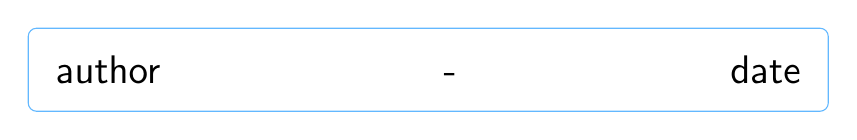
\begin{tikzpicture}
\node[rectangle,rounded corners=3pt,inner sep=10pt,draw=SteelBlue1,text width= 0.78\textwidth] {\Large \@author \hfill-\hfill\@date};
\end{tikzpicture}
\end{minipage}
%\bigskip%\bigskip
}%
\makeatother

% custom section
\newcommand*\sectionlabel{}
\titleformat{\section}
  {\gdef\sectionlabel{}
   \normalfont\sffamily\Large\bfseries\scshape}
  {\gdef\sectionlabel{\thesection\ }}{0pt}
  {
\noindent
\begin{tikzpicture}
\node[rectangle,rounded corners=3pt,inner sep=4pt,fill=DodgerBlue4,text width= 0.95\columnwidth] {\color{white}\sectionlabel#1};
\end{tikzpicture}
  }
\titlespacing*{\section}{0pt}{5pt}{2.5pt}

% custom subsection
\newcommand*\subsectionlabel{}
\titleformat{\subsection}{\normalfont\sffamily\bfseries\scshape}{\subsectionlabel}{0pt}{
\noindent
\begin{tikzpicture}
\node[rectangle,rounded corners=4pt,inner sep=3pt,fill=DodgerBlue3,text width= 0.95\columnwidth] {\color{white}\subsectionlabel#1};
\end{tikzpicture}
}
\titlespacing*{\subsection}{0pt}{5pt}{2.5pt}

% custom subsubsection
\newcommand*\subsubsectionlabel{}
\titleformat{\subsubsection}{\normalfont\sffamily\small\bfseries\scshape}{\subsubsectionlabel}{0pt}{
\noindent
\begin{tikzpicture}
\node[rectangle,rounded corners=3pt,inner sep=3pt,fill=blue!50!yellow,text width= 0.95\columnwidth] {\color{white}\subsubsectionlabel#1};
\end{tikzpicture}
}
\titlespacing*{\subsubsection}{0pt}{5pt}{2.5pt}


\title{MAT265 - Équations différentielles}
\author{Examen Final}
\date{Été 2018}

%\linespread{1.3}

\begin{document}
\maketitle

\begin{multicols*}{2}

%\input{ed_lin_1er}

%\input{eq_lin_2e}

%\input{problemes}

%\input{application}

%\section{Série de Puissances}
\vspace{-1\baselineskip}
\begin{gather*}
p(x)y^{\prime\prime} +q(x)y^{\prime}+r(x)y=0 ~~~  \left\{ \begin{array}{rcl}
y(x_0)& =& y_0\\
y^{\prime}(x_0) & = & y^{\prime}_0
\end{array} \right.
\end{gather*}
\centering
\begin{tabular}{rl}\hline
    $x_0$ & $x_0$ \\
    Points singuliers & \(p(x)=0\) ~~``\(\mathbf{cSolve}()\)'' \\
    Si partie imaginaire & \(R=\sqrt{(x_0)^2 + \beta^2}\)\\
    Sinon & \(R=x_0-\alpha\)\\
    Intervalle de convergence & \(I=]\,x_0-R,\; x_0+R\,[\)\\\hline
\end{tabular}
\\\raggedright
Solution de l'É.D.: ( sauf si $R=0 \Rightarrow I=\emptyset$ )
\vspace{-0.25em}
\begin{equation*}
    \left. y(x)=\sum^{\infty}_{n=0} a_n (x-x_0)^n  \;\;\right| x \in ]\,x_0-R,\; x_0+R\,[
\end{equation*}
\vspace{-0.25em}
\begin{enumerate}[nosep]
    \item Si $x_0 \neq 0$, on pose $v=x\pm x_0$
    \item On remplace $y \longleftarrow \sum{ a_n x^n}$
    \item On obtient:
\end{enumerate}
\centering
\(
    P\sum{ (n-1)n a_n x^{n-2}} +Q\sum{n a_n x^{n-1}}+R\sum{a_n x^n}=0
\)\\\raggedright

\begin{enumerate}[nosep]
\setcounter{enumi}{3}
    \item On remplace $n\leftarrow (n+2), n\leftarrow (n+1)$
    \item On isole le $x^n$ \hspace{1em}[Attention: $x\times x^{n-2}\Rightarrow x^{n-1}$]
    \item On élimine $\Sigma$ et $x^n \;\Rightarrow\;(\Delta_{n+2}\; a_{n+2}+\Delta_{n+1}\; a_{n+1})= 0$
    \item On isole le coefficient d'indice supérieur $a_{n+2}$
\end{enumerate}

\centering
\(
    a_{n+2} = \Delta_{n+1}\; a_{n+1}+\Delta_{n}\; a_{n}
\)
\begin{enumerate}[nosep]
\setcounter{enumi}{7}
    \item On remplace $n\leftarrow (n-2)$
\end{enumerate}
\centering
\(
    a_{n} = \Delta_{n-1}\; a_{n-1}+\Delta_{n-2}\; a_{n-2}
\)

\subsection{Formule de récurrence}
% \vspace{-.75em}
\begin{equation*}
   a_n= \left\{ \begin{array}{ll}
        0 & n<0 \\
        a_0=y(x_0) & n=0\\
        a_1=y^{\prime}(x_0) & n=1\\
        a_n & n\geq 2
    \end{array}\right.
\end{equation*}
% \begin{equation*}
%     y(x)= 
% \end{equation*}
% \vspace{-.75em}

\begin{enumerate}[nosep]
\setcounter{enumi}{8}
    \item On assemble la formule de sommation $y(x)=\Sigma\cdots$
    \item On donne les $n$ premier termes de l'É.D.
\end{enumerate}

\subsubsection{TI}
% \vspace{-.75em}
\begin{equation*}
    a(n):=\left\{ \begin{array}{ll}
        0 & n<0 \\
        a_0=y(x_0) & n=0\\
        a_1=y^{\prime}(x_0) & n=1\\
        \Delta_{n-2}\: a(n-2)+\Delta_{n-1}\; a(n-1) & n\geq 2
    \end{array}\right.
\end{equation*}\\
\vspace{.125em}
{\centering\(\mathbf{seq}(Expr,Var,Inf,Sup)\)}
\vspace{.125em}
% \vspace{-.75em}

\subsection{Calcul des coefficients}
\vspace{-.75\baselineskip}
\begin{align*}
    a_0 &= \frac{2}{P}+\int_{c-\frac{P}{2}}^{c+\frac{P}{2}} y(x) \:dx \\
    a_n &= \frac{2}{P}+\int_{c-\frac{P}{2}}^{c+\frac{P}{2}} y(x)\cos\bigg(n\frac{2\pi}{P}x\bigg) \:dx \\
    b_n &= \frac{2}{P}+\int_{c-\frac{P}{2}}^{c+\frac{P}{2}} y(x)\sin\bigg(n\frac{2\pi}{P}x\bigg) \:dx
\end{align*}
\subsubsection{TI}
\centering
\(
    \mathbf{a0}(c,p,x,fn)\hspace{1em}    \mathbf{an}(c,p,x,fn)\hspace{1em}    \mathbf{bn}(c,p,x,fn) 
\)\\
\raggedright
Représentation graphique
\begin{align*}
    f1(x) &= y(x)\,\mathbf{mod}(x,P)\\
    f2(x)&=y(x)
\end{align*}


\section{Fonction définie par morceaux}
\vspace{-2.5\baselineskip}
\begin{gather*}
f(t) = \left\{ \begin{array}{cc}
 0 & t < \pi \\
 f(t) & t \geq \pi
  \end{array}
  \right.
\;\;\Longleftrightarrow\;\; f(t)u(t-\pi)
\end{gather*}\vspace{-\baselineskip}\\
Inverse (exemple):
\begin{align*}
 y(t)   =&\; (e^{-3t}+e^t)u(t)\tag{1}\\
        &\quad+\frac{1}{4}(e^{t-1}-e^{-3t+3})u(t-1)\tag{2}\\
        &\qquad-\frac{1}{4}(e^{t-2}-e^{-3t+6})u(t-2)\tag{3}
\end{align*}
\begin{equation*}
y(t) = \left\{ \begin{array}{cc}
 0 & t < 0 \\
 (1) & 0\leq t<1\\
 (1)+(2) & 1\leq t<2\\
 (1)+(2)+(3) & t\geq 2
  \end{array}
  \right.
\end{equation*}

\subsubsection{TI}
\centering
\(f(t)\:\mathbf{step}(t-a)\)\\\raggedright
\section{Transformée de Laplace}
%% TODO Ajouter quelque chose p/r au coefficients. As+B
%Linéarité

\subsection{Propriétés}
\noindent
Linéarité \hspace{1em}\(\mathcal{L}\left\{\alpha f(t)+\beta g(t)\right\}= \alpha F(s) + \beta G(s)\)

\subsection{Transformée inverse}

Si $x_0 \neq 0$, on pose \(v=x\pm \Delta x\)\\\raggedright
\begin{enumerate}[nosep]
    \item Mettre en évidence les \(\mathbf{e}^{-at}\)
    \item Modifier l'équation (expand, propFrac)
    \item Résoudre l'équation
\end{enumerate}
Si on veut la réponse sous la forme \(A\sin(\omega t+\phi)\)\\\raggedright

\subsubsection{TI}
\centering
\( \mathbf{expand}() \hspace{1em} \mathbf{propFrac}() \hspace{1em} \mathbf{completeSquare}() \)\\
\(
    \mathbf{tCollect}()\hspace{1em}    \mathbf{tExpand}()\hspace{1em}    \mathbf{ilaplace}() 
\)\\
\raggedright
\section{Série de Puissances}
\vspace{-1\baselineskip}
\begin{gather*}
p(x)y^{\prime\prime} +q(x)y^{\prime}+r(x)y=0 ~~~  \left\{ \begin{array}{rcl}
y(x_0)& =& y_0\\
y^{\prime}(x_0) & = & y^{\prime}_0
\end{array} \right.
\end{gather*}
\centering
\begin{tabular}{rl}\hline
    $x_0$ & $x_0$ \\
    Points singuliers & \(p(x)=0\) ~~``\(\mathbf{cSolve}()\)'' \\
    Si partie imaginaire & \(R=\sqrt{(x_0)^2 + \beta^2}\)\\
    Sinon & \(R=x_0-\alpha\)\\
    Intervalle de convergence & \(I=]\,x_0-R,\; x_0+R\,[\)\\\hline
\end{tabular}
\\\raggedright
Solution de l'É.D.: ( sauf si $R=0 \Rightarrow I=\emptyset$ )
\vspace{-0.25em}
\begin{equation*}
    \left. y(x)=\sum^{\infty}_{n=0} a_n (x-x_0)^n  \;\;\right| x \in ]\,x_0-R,\; x_0+R\,[
\end{equation*}
\vspace{-0.25em}
\begin{enumerate}[nosep]
    \item Si $x_0 \neq 0$, on pose $v=x\pm x_0$
    \item On remplace $y \longleftarrow \sum{ a_n x^n}$
    \item On obtient:
\end{enumerate}
\centering
\(
    P\sum{ (n-1)n a_n x^{n-2}} +Q\sum{n a_n x^{n-1}}+R\sum{a_n x^n}=0
\)\\\raggedright

\begin{enumerate}[nosep]
\setcounter{enumi}{3}
    \item On remplace $n\leftarrow (n+2), n\leftarrow (n+1)$
    \item On isole le $x^n$ \hspace{1em}[Attention: $x\times x^{n-2}\Rightarrow x^{n-1}$]
    \item On élimine $\Sigma$ et $x^n \;\Rightarrow\;(\Delta_{n+2}\; a_{n+2}+\Delta_{n+1}\; a_{n+1})= 0$
    \item On isole le coefficient d'indice supérieur $a_{n+2}$
\end{enumerate}

\centering
\(
    a_{n+2} = \Delta_{n+1}\; a_{n+1}+\Delta_{n}\; a_{n}
\)
\begin{enumerate}[nosep]
\setcounter{enumi}{7}
    \item On remplace $n\leftarrow (n-2)$
\end{enumerate}
\centering
\(
    a_{n} = \Delta_{n-1}\; a_{n-1}+\Delta_{n-2}\; a_{n-2}
\)

\subsection{Formule de récurrence}
% \vspace{-.75em}
\begin{equation*}
   a_n= \left\{ \begin{array}{ll}
        0 & n<0 \\
        a_0=y(x_0) & n=0\\
        a_1=y^{\prime}(x_0) & n=1\\
        a_n & n\geq 2
    \end{array}\right.
\end{equation*}
% \begin{equation*}
%     y(x)= 
% \end{equation*}
% \vspace{-.75em}

\begin{enumerate}[nosep]
\setcounter{enumi}{8}
    \item On assemble la formule de sommation $y(x)=\Sigma\cdots$
    \item On donne les $n$ premier termes de l'É.D.
\end{enumerate}

\subsubsection{TI}
% \vspace{-.75em}
\begin{equation*}
    a(n):=\left\{ \begin{array}{ll}
        0 & n<0 \\
        a_0=y(x_0) & n=0\\
        a_1=y^{\prime}(x_0) & n=1\\
        \Delta_{n-2}\: a(n-2)+\Delta_{n-1}\; a(n-1) & n\geq 2
    \end{array}\right.
\end{equation*}\\
\vspace{.125em}
{\centering\(\mathbf{seq}(Expr,Var,Inf,Sup)\)}
\vspace{.125em}
% \vspace{-.75em}

\subsection{Calcul des coefficients}
\vspace{-.75\baselineskip}
\begin{align*}
    a_0 &= \frac{2}{P}+\int_{c-\frac{P}{2}}^{c+\frac{P}{2}} y(x) \:dx \\
    a_n &= \frac{2}{P}+\int_{c-\frac{P}{2}}^{c+\frac{P}{2}} y(x)\cos\bigg(n\frac{2\pi}{P}x\bigg) \:dx \\
    b_n &= \frac{2}{P}+\int_{c-\frac{P}{2}}^{c+\frac{P}{2}} y(x)\sin\bigg(n\frac{2\pi}{P}x\bigg) \:dx
\end{align*}
\subsubsection{TI}
\centering
\(
    \mathbf{a0}(c,p,x,fn)\hspace{1em}    \mathbf{an}(c,p,x,fn)\hspace{1em}    \mathbf{bn}(c,p,x,fn) 
\)\\
\raggedright
Représentation graphique
\begin{align*}
    f1(x) &= y(x)\,\mathbf{mod}(x,P)\\
    f2(x)&=y(x)
\end{align*}

\section{Séries de Fourier}
\subsection{Calcul des coefficients}

On pose\hspace{1em}\(
  g(x) = \frac{a_0}{2} + \sum_{n=1}^{\infty} a_n \cos(n\,\omega\,x) +b_n \sin(n\, \omega \,x)
\)\\
\raggedright
On calcule les coefficients:
\begin{align*}
  a_0 &= \frac{2}{L} \int^L_0 g(x) \:dx \\
  a_n &= \frac{2}{L} \int^L_0 g(x)\cos(n\,\omega\,x) \:dx \\
  b_n &= \frac{2}{L} \int^L_0 g(x)\sin(n\,\omega\,x) \:dx
\end{align*}
Paramètres
\begin{tabular}{rcl}
$P$ & : & Période de $g(x)$\\
$L$ & = & $P / 2$\\
$\omega$ & = & $2\pi / P \Leftrightarrow 2\pi/2L \Leftrightarrow  \pi/L$ 
\end{tabular}

\subsection{Avec table}

\begin{enumerate}[nosep]
  \item Tracer le graphique de g(x)
  \item Trouver une fonction similaire dans la table
  \item Écrire la valeur des paramètres
  \item Calculer les proportions
\end{enumerate}

Paramètres
\begin{tabular}{rcl}
\(A_g\) & : & Amplitude de \(g(x)\)\\
\(P_g\) & : & Période de \(f(x)\)\\
\(H\) & : & Écart en \(y\)\\
\(c\) & : & Écart en \(x\)\\
\(A_f\) & : & Amplitude de \( f(x) \)\\
\(P_f\) & : & Période de \(f(x)\)
\end{tabular}

\begin{equation*}
  g(x)= H \pm \frac{A_g}{A_f} f\bigg( \frac{P_f}{P_g} (x-c) \bigg)
\end{equation*}

On remplace dans la série \( f(x) \mid x \leftarrow \frac{P_f}{P_g} (x-c) \)

\subsection{Prolongement périodique}
\begin{equation*}
  f(x) = \frac{a_0}{2} + \sum_{n=1}^{\infty} a_n \cos(n \frac{\pi}{L}x) +b_n \sin(n \frac{\pi}{L}x)
\end{equation*}

\begin{tabular}{llll}
    Prolong. ordinaire & \(a_0\) & \(a_n\) & \(b_n\)\\
    Prolong. pair & \(a_0\) & \(a_n\) & \(b_n=0\) \\
    Prolong. impair & \(a_0=0\) & \(a_n=0\) & \(b_n\)
\end{tabular}
\subsubsection{TI}
%\centering
\(\mathbf{prlgp}(type,l,x,fn)\mid\) type: \(o,p,i\) \hfill\(\mathbf{prlgp\_dev}(type,l,x,fn)\)\\
\centering
\(
    \mathbf{a0p}(L,x,fn)\hspace{1em}    \mathbf{anp}(L,x,fn)\hspace{1em}    \mathbf{bnp}(L,x,fn) 
\)\\
%Applications
\section{Application des É.D. d'ordre 2}
\subsubsection{TI}
\centering
\(\mathbf{solver}(\left\{p,q,r\right\}=g(t),t,y,t_0,y_0,y^{\prime}_0)\)\\

\subsection{Type de régime}
\begin{tabular}{ll}
Régime libre & \(g(t)=0\)\\
Régime non amorti & \(g(t)=0\) et \(b=0\)\\
Régime libre sous-amorti & \(g(t)=0\) et \(b<2\sqrt{c} \rightarrow \Delta <0\)\\
Régime libre sur-amorti & \(g(t)=0\) et \(b>2\sqrt{c} \rightarrow \Delta >0\)\\
Régime libre critique & \(g(t)=0\) et \(b=2\sqrt{c} \rightarrow \Delta = 0\)\\
Régime forcé & \(g(t)\neq 0\)
\end{tabular}
\raggedright

\subsection{Mouv. harmonique (Ressorts)}
\vspace{-1\baselineskip}
\begin{gather*}
m y^{\prime\prime} + \beta y^{\prime} + ky = g(t) \;\;\Longleftrightarrow\;\;
y^{\prime\prime} + \frac{\beta}{m} y^{\prime} + \frac{k}{m}y = \frac{g(t)}{m}
\end{gather*}
Paramètres
\begin{tabular}{rll}
  $m$ & masse & [$kg$]\\
  $\beta$ & coefficient d'amortissement & [$N\cdot s/m$]\\
  $k$ & constante de rappel du ressort & [$N/m$]\\
  $g(t)$ & force externe & [$N$]\\
  $y(t)$ & position p/r à équilibre & [$m$]\\
  $v(t)=\frac{dy}{dt}$ & vitesse & [$m/s$]\\
  $a(t)=\frac{dv}{dt}$ & accélération & [$m/s^2$]
\end{tabular}


\subsubsection{TI}
\centering
\(\mathbf{ressort}(m,b,k,f,y_0,v_0)\)\\
\subsection{Circuit RLC}
{\centering
\resizebox{.1\textwidth}{!}{
\begin{circuitikz}
    \draw (0,0)
    to[R, l=$R$] (2,0)
    to[L, l=$L$] (2,-2)
    to[C, l=$C$] (0,-2)
    to[V, l=$V$, invert] (0,0);
\end{circuitikz}
}
}
\\\raggedright
Voltage au capaciteur:
{\centering
%\begin{gather*}
\(
LC V_c^{\prime\prime} + RC V_c^{\prime} + V_c = V(t)\Longleftrightarrow
V_c^{\prime\prime} + \frac{R}{L} V_c^{\prime} + \frac{1}{LC}V_c = \frac{V(t)}{LC}
\)}\\
%\end{gather*}
Courant:
{\centering\(
%\begin{gather*}
L i^{\prime\prime} + R i^{\prime} + \frac{1}{C}i = E(t)\;\;\Longleftrightarrow\;\;
i^{\prime\prime} + \frac{R}{L} i^{\prime} + \frac{1}{LC}i = \frac{E(t)}{L}
% \end{gather*}
\)}\\
Avec:
\begin{tabular}{rlc}
  $R$ & résistance & [$\Omega$] \\
  $L$ & inductance & [$H$]\\
  $C$ & capacité & [$F$]\\
  $E(t)=V(t)$ & source de puissance & [$V$]\\
  $V_c(t)*C = i(t_0)$ & courant à $t_0$ & [$A$]\\
  $V_c(t_0)=i^{\prime}(t_0)$ & voltage au capaciteur à $t_0$ & [$V$]
\end{tabular}


\subsubsection{TI}
\centering
\(\mathbf{circuit}(R,L,C,E,Vc_0,I_0)\)\\


\section{Algorithme de Runge-Kutta}
\raggedright
\subsection{$1^{\mathrm{er}}$ ordre}

\begin{equation*}
    \left\{ \begin{array}{rcl}
        y^{\prime} & = & x^2+y^2 \\
        y(x_0) & = & y_0
    \end{array}\right.
\end{equation*}

\subsubsection{TI}
\menu[,]{Menu,3,8}
\begin{equation*}
    \left\{ \begin{array}{rcl}
        y1^{\prime} & = & x^2+y1^2 \\
        (x_0,y1_0) & = & y_0
    \end{array}\right.
\end{equation*}

Puis: \menu[,]{\ldots,Runge-Kutta, Tol. erreur: 0.0001, Champ: Aucun}

\subsection{$2^{\mathrm{e}}$ ordre}

\begin{equation*}
    \left\{ \begin{array}{rcl}
        (x-5)y^{\prime\prime} +xy^{\prime}+3y & = & 0 \\
        y(x_0) & = & y_0\\
        y^{\prime}(x_0) & = & y^{\prime}_0
    \end{array}\right.
\end{equation*}

%\raggedright

On transforme l'É.D. en É.D. du $1^{\mathrm{er}}$ ordre.\\
On pose: \( y=y_1 \;\mathrm{ et }\; y^{\prime}=y_2 \Longleftrightarrow y^{\prime\prime}=y^{\prime}_2 \)\\
\subsubsection{TI}
\centering
\(\mathbf{de2to1}(Py^{\prime\prime} +Qy^{\prime}+Ry = 0)\)\\\raggedright

\menu[,]{Menu,3,8}
\begin{equation*}
    \left\{ \begin{array}{rcl}
        y1^{\prime} & = & y2 \\
        (x_0,y1_0) & = & y_0\\
        y2^{\prime} & = & y_2^{\prime} \quad\mathrm{(E.D.}\ 1^{er}\ \mathrm{ ordre)}\\
        (x_0, y2_0) & = & y^{\prime}_0
    \end{array}\right.
\end{equation*}

Puis: \menu[,]{\ldots,Runge-Kutta, Tol. erreur: 0.0001, Champ: Aucun}

\subsection{Éditer les valeurs dans le tableau}

\begin{tabular}{cl}
\keys{ctrl+T} & Afficher/Quitter la table des valeurs\\
\keys{menu+2+5} & Paramètres de la table
\end{tabular}
% \includepdf[pages=-]{formulaire-algebre-trigo.pdf}
% \includepdf[pages=-]{laplace-table.pdf}
% \includepdf[pages=-]{Fourier-table.pdf}
% \includepdf[pages=-]{265godsheet.pdf}

\end{multicols*}

\end{document}
